
\documentclass{article}
\usepackage[margin=1in]{geometry}
\usepackage{graphicx}
\usepackage[fleqn]{amsmath}
\begin{document}
   \begin{flushright}
      \Large\textbf{Steven Murr}\\
      \large\textit{HW 1.2}
   \end{flushright}
\begin{flushleft}
\setlength\parindent{0pt}1) You cannot edit a protected Wikipedia entry unless you are an administrator.\\
Express your answer in terms of:\\
\setlength\parindent{24pt}e: "You can edit a protected Wikipedia entry" \\
\setlength\parindent{24pt}a: "You are an administrator."\\
\setlength\parindent{48pt} $\neg a \rightarrow \neg e$ \\
\setlength\parindent{48pt} $e \rightarrow a$ \\
\setlength\parindent{48pt} The contrapositive always has the same truth value.  Hence why 
\setlength\parindent{48pt} $e \rightarrow a$ is equivalent\\
\setlength\parindent{0pt}3) You can graduate only if you have completed the requirements of your major and you do not owe money to the university and you do not have an overdue library book.  \\
Express your answer in terms of\\
\setlength\parindent{24pt}g: "You can graduate," \\
\setlength\parindent{24pt}m: "You owe money to the university," \\
\setlength\parindent{24pt}r: "You have completed the requirements of your major," \\
\setlength\parindent{24pt}b: "You have an overdue library book."\\
\setlength\parindent{48pt} $g \rightarrow (r \land \neg m) \land \neg b$ \\
\setlength\parindent{0pt}7) Express these system specifications using the the following propositions with logical connectives (including negations)\\ 
\setlength\parindent{24pt}p: "The message is scanned for viruses" \\
\setlength\parindent{24pt}q: "The message was sent from an unknown system"\\
\setlength\parindent{48pt}a) "The message is scanned for viruses whenever the message was sent from \\
\setlength\parindent{48pt}an unknown system."\\
\setlength\parindent{55pt}$q \rightarrow p$\\

\setlength\parindent{48pt}b) "The message was sent from an unknown system but \\
\setlength\parindent{48pt}it was not scanned for viruses."\\
\setlength\parindent{55pt}$q \land \neg p$\\
\setlength\parindent{48pt}c) "It is necessary to scan the message for viruses whenever\\
\setlength\parindent{48pt}it was sent from an unknown system."\\
\setlength\parindent{55pt}$q \rightarrow p$\\
\setlength\parindent{48pt}d) "When a message is not sent from an unknown system \\
\setlength\parindent{48pt}it is not scanned for viruses."\\
\setlength\parindent{55pt}$\neg q \rightarrow \neg p$\\
\setlength\parindent{0pt}17) When three professors are seated in a restaurant, the hostess asks them: "Does every want coffee?" The first professor says: "I do not know."  The second professor then says: "I do not know." The hostess comes back and gives coffee to the professors who want it.  How did she figure out who wanted coffee?" \\
~\\The hostess asks the question "Does \underline{everyone} want coffee?"  The third professor is the only one to explicitly say "No, not everyone wants coffee."  He is simultaneously turning down coffee and inferring that the other professors are having coffee by stating that "not everyone wants coffee." \\

~\\\setlength\parindent{0pt}18) When planning a party you want to know whom to invite.  Among the people you would like to invite are three touchy friends.  You know that if Jasmine attends, she will become unhappy if Samir is there, Samir will attend only if Kanti will be there, and Kanti will not attend unless Jasmine also does.  Which combinations of these three friends can you invite so as not to make someone unhappy?\\
~\\
First we translate the aforementioned statements into symbolic logic using j, s and k for Jasime, Samir and Kanti.\\
$j \rightarrow \neg s = $ If Jasmine goes, then Samir isn't going. \\
$s \rightarrow k = $ If Samir attends then Kanti will be there.\\
$\neg j \rightarrow \neg k$ If Jasmine doesn't attend, then Kanti won't attend. \\ 
~\\
We are trying to find combinations of these three friends to invite in which Jasmine is happy.  So we initially start by making $\neg s$ True which also allows $j$ to be True because Jasmine can now go and be happy.  In the second case, if $\neg s $ is True then s is false, allowing k to be either True or False.  In this case,  $k$ will be true.  In the third case, $\neg k $ evaluates to false (because we accepted k to be true) and $\neg j $ evaluates to false (because we accepted j to be true) leading to the system being consistent.\\
Therefore, the following combinations satisfy the system:\\
~\\I) None of the friends go\\
II) Only Jasmine goes\\
III) Only Jasmine and Kanti goes\\
~\\
\setlength\parindent{0pt}20) A says "The two of us are both knights" and B says "A is a knave." \\
If B is telling the truth and is thus a knight then A would have to be a Knave.  Since A's statement was "the TWO of us are both knights" it is technically False.  Thus, A is a Knave and B is a Knight. \\
~\\
\setlength\parindent{0pt}33) Steve would like to determine the relative salaries of three coworkers using two facts.  First, he knows that if Fred is not highest paid of the three, then Janice is.  Second, he knows that if Janice is not the lowest paid, then Maggie is paid the most.  Is it possible to determine the relative salaries of Fred, Maggie, and Janice from what Steve knows?  If so, who is paid the most and who the least?  Explain your reasoning.\\
~\\
First, make statements sound more explicit.\\
If Fred is not the highest paid then Janice is not the highest paid.\\
If Janice is not the lowest paid, then Maggie is paid the most.\\
~\\
If Fred is not the highest paid is false, then Janice is the lowest paid.  Then since Janice is the lowest paid, the second statement fails so Maggie is not paid the most.  The final salary breakdown in descending order:\\
$Fred > Maggie > Janice$\\
** Inversely, if Fred is not the highest paid is True, then Janice is the lowest paid.  Then Janice being the lowest paid fails the next statement therefore Maggie can't be paid the most and we are unable to infer the proper order.  \\
~\\
\setlength\parindent{0pt}40) Find the output of each of these combinatorial circuits.\\
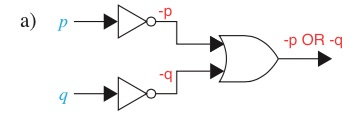
\includegraphics[width=90mm]{cb1.jpg} \\
\setlength\parindent{24pt}Final circuit $\neg p \lor \neg q$ \\
\setlength\parindent{0pt}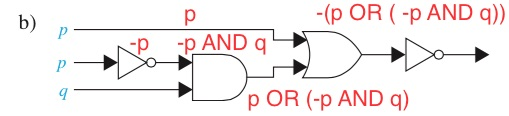
\includegraphics[width=90mm]{cb2.jpg} \\
\setlength\parindent{24pt}Final circuit $\neg (p \lor (\neg p \land q))$ \\
~\\
\setlength\parindent{0pt}41) Find the output of each of these combinatorial circuits.\\
\setlength\parindent{0pt}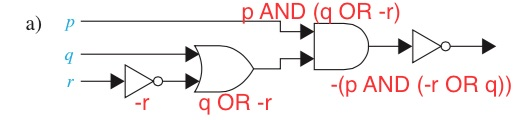
\includegraphics[width=90mm]{cb3.jpg} \\
\setlength\parindent{24pt}Final circuit $\neg (p \land (\neg r \lor q))$ \\
\setlength\parindent{0pt}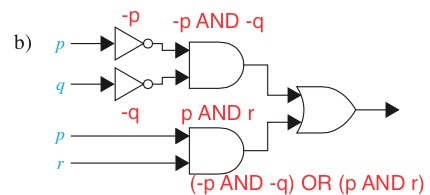
\includegraphics[width=90mm]{cb4.jpg} \\
\setlength\parindent{24pt}Final circuit $(\neg p \land \neg q) \land (p \land r)$ \\

\end{flushleft}
\end{document}